\documentclass{article}
\usepackage{braket}
\usepackage{amsmath}
\usepackage{amssymb}
\usepackage{hyperref}
\usepackage{graphicx}
\usepackage{kotex}
\newcommand{\bfit}[1]{\textit{\textbf{#1}}}
\begin{document}
\textbf{\Large Chapter 5\\ Bloch Sphere, Quantum Gates, and Pauli Matrics}
\\\\\\
\textbf{\large 5.1 Introduction}\\\\
In this chapter, we will introduce the Bloch sphere to which a 2D complex
space of a single qubit is mapped. The Bloch sphere is embedded in the real 
3D space. As a result, the manipulation of a qubit by a quantum gate is equibalent to a rotation on the
Bloch sphere. We will show the rotation matrix of an arbitarry quantum
gate and its decomposition. Then we will discuss Pauli matrices and their properties.
Pauli matrices are the generators of rotations. Understanding the properties of the
Pauli matrices helps us derive many important equations. Finally, we will discuss
the universal sets of quantum gates which can be used to implement all qunatum gates.
\\\\
\bfit{\large 5.1.1 Learning Outcomes}
\\\\
Understand the nuature of the Bloch sphere and its relationship to real 3D space;
be able to construct the rotation matrix of any given rotation on the Bloch sphere;
understand the properties of Pauli matrices.\\\\
\bfit{\large 5.1.2 Teaching Videos}\\\\
$\bullet$ Search for Ch5 in this playlist\\
- \url{http://tinyurl.com/3yhze3jn}\\\\
$\bullet$ Other videos\\
- \url{http://youtu.be/IRoYYJM8Gq8}\\
- \url{http://youtu.be/MLkDyY91_GU}\\
- \url{http://youtu.be/JR2jRCeTHDc}\\
- \url{http://youtu.be/MTmQKP_9iJ0}\\
\\\\
\textbf{\large 5.2 Bloch Sphere}\\\\
A single-qubit state, $\ket{\psi}$, can be expressed as a linear combination of the two basis
states, $\ket{0}$ and $\ket{1}$. Therefore, $\ket{\psi}=\alpha\ket{0}+\beta\ket{1}$. $\alpha$ and $\beta$ are complex numbers.
Each complex number has a manitude and a phase ($\alpha=|\alpha|e^{i\delta_{\alpha}}$ and $\beta=|\beta|e^{i\delta_{\beta}}$).
Therefore, we need to fix four real numbers in order to fix $\alpha$ and $\beta$ and, thus $\ket{\psi}$.
As a result, $\ket{\psi}$ has four \textbf{degrees of freedom (DOFs)}. So, it is impossible to
visualize the 2D complex Hilber space of a 1-qubit system in our real 3D space.

However, since a physical state vector must be normalized (Sect. 2.3.4), the DOF
is reduced to 3 due to the constraint that $|\alpha|^2+|\beta|^2=1$. 
We can set $|\alpha|=\cos{\frac{\theta}{2}}$ and $|\beta|=\sin{\frac{\theta}{2}}$ as 
$(\cos{\frac{\theta}{2}})^2+(\sin{\frac{\theta}{2}})^2=1$ so that we use the parameter
$\theta$ instead of $|\alpha|$ and $|\beta|$. We can then write the qubit state as
\begin{align} \label{eq 5.1}
    \begin{split}
        \ket{\psi} &= \alpha\ket{0}+\beta\ket{1},\\
        &= |\alpha|e^{i\delta_{\alpha}}\ket{0}+\beta|e^{i\delta_{\beta}}\ket{1},\\
        &= \cos{\frac{\theta}{2}}e^{i\delta_{\alpha}}\ket{0}+\sin{\frac{\theta}{2}}e^{i\delta_{\beta}}\ket{1},\\
        &=e^{i(\delta_{\alpha}+\delta_{\beta})/2}(\cos{\frac{\theta}{2}}e^{i(\delta_{\alpha}-\delta_{\beta})/2}\ket{0}
        +\sin{\frac{\theta}{2}}e^{i(-\delta_{\alpha}+\delta_{\beta})/2}\ket{1}),\\
        &=e^{i(\delta_{\alpha}+\delta_{\beta})/2}(\cos{\frac{\theta}{2}}e^{-i\phi/2}\ket{0}
        +\sin{\frac{\theta}{2}}e^{i\phi/2}\ket{1}),\\
        &=e^{i\gamma}(\cos{\frac{\theta}{2}}e^{-i\phi/2}\ket{0}+\sin{\frac{\theta}{2}}e^{i\phi/2}\ket{1}).
    \end{split}\tag{5.1}
\end{align}\\
We have performed some variable changes and substitutions. For example, we introduced
$\gamma=(\delta_{\alpha}+\delta_{\beta})/2$ and $\phi=\delta_{\beta}-\delta_{\alpha}$.
Now, $\ket{\psi}$ is described by three \textit{real} parameters, $\gamma, \theta,$ and $\phi$. e$^{i\gamma}$ gives the global phase of the state. It is not important when 
the qubit is isolated bcause the inner product ro the expectation values of the state will no chnage. For 
example, if a phase of e$^{i\gamma^{\prime}}$ is added to state $\ket{\psi}$ so it becomes 
$\ket{\psi^{\prime}}=e^{i\gamma}\ket{\psi}$ and we perform a measurement corresponding
to an observable \bfit{M},  the expectation value (Eq.(3.31)) is
\begin{equation} \label{eq 5.2}
    \braket{\psi^{\prime}|\bfit{M}|\psi^{\prime}}=\braket{\psi|e^{-i\gamma^{\prime}}\bfit{M}e^{i\gamma^{\prime}}|\psi}
    =\braket{\psi|\bfit{M}|\psi} \tag{5.2}
\end{equation}
\\
\begin{center}
    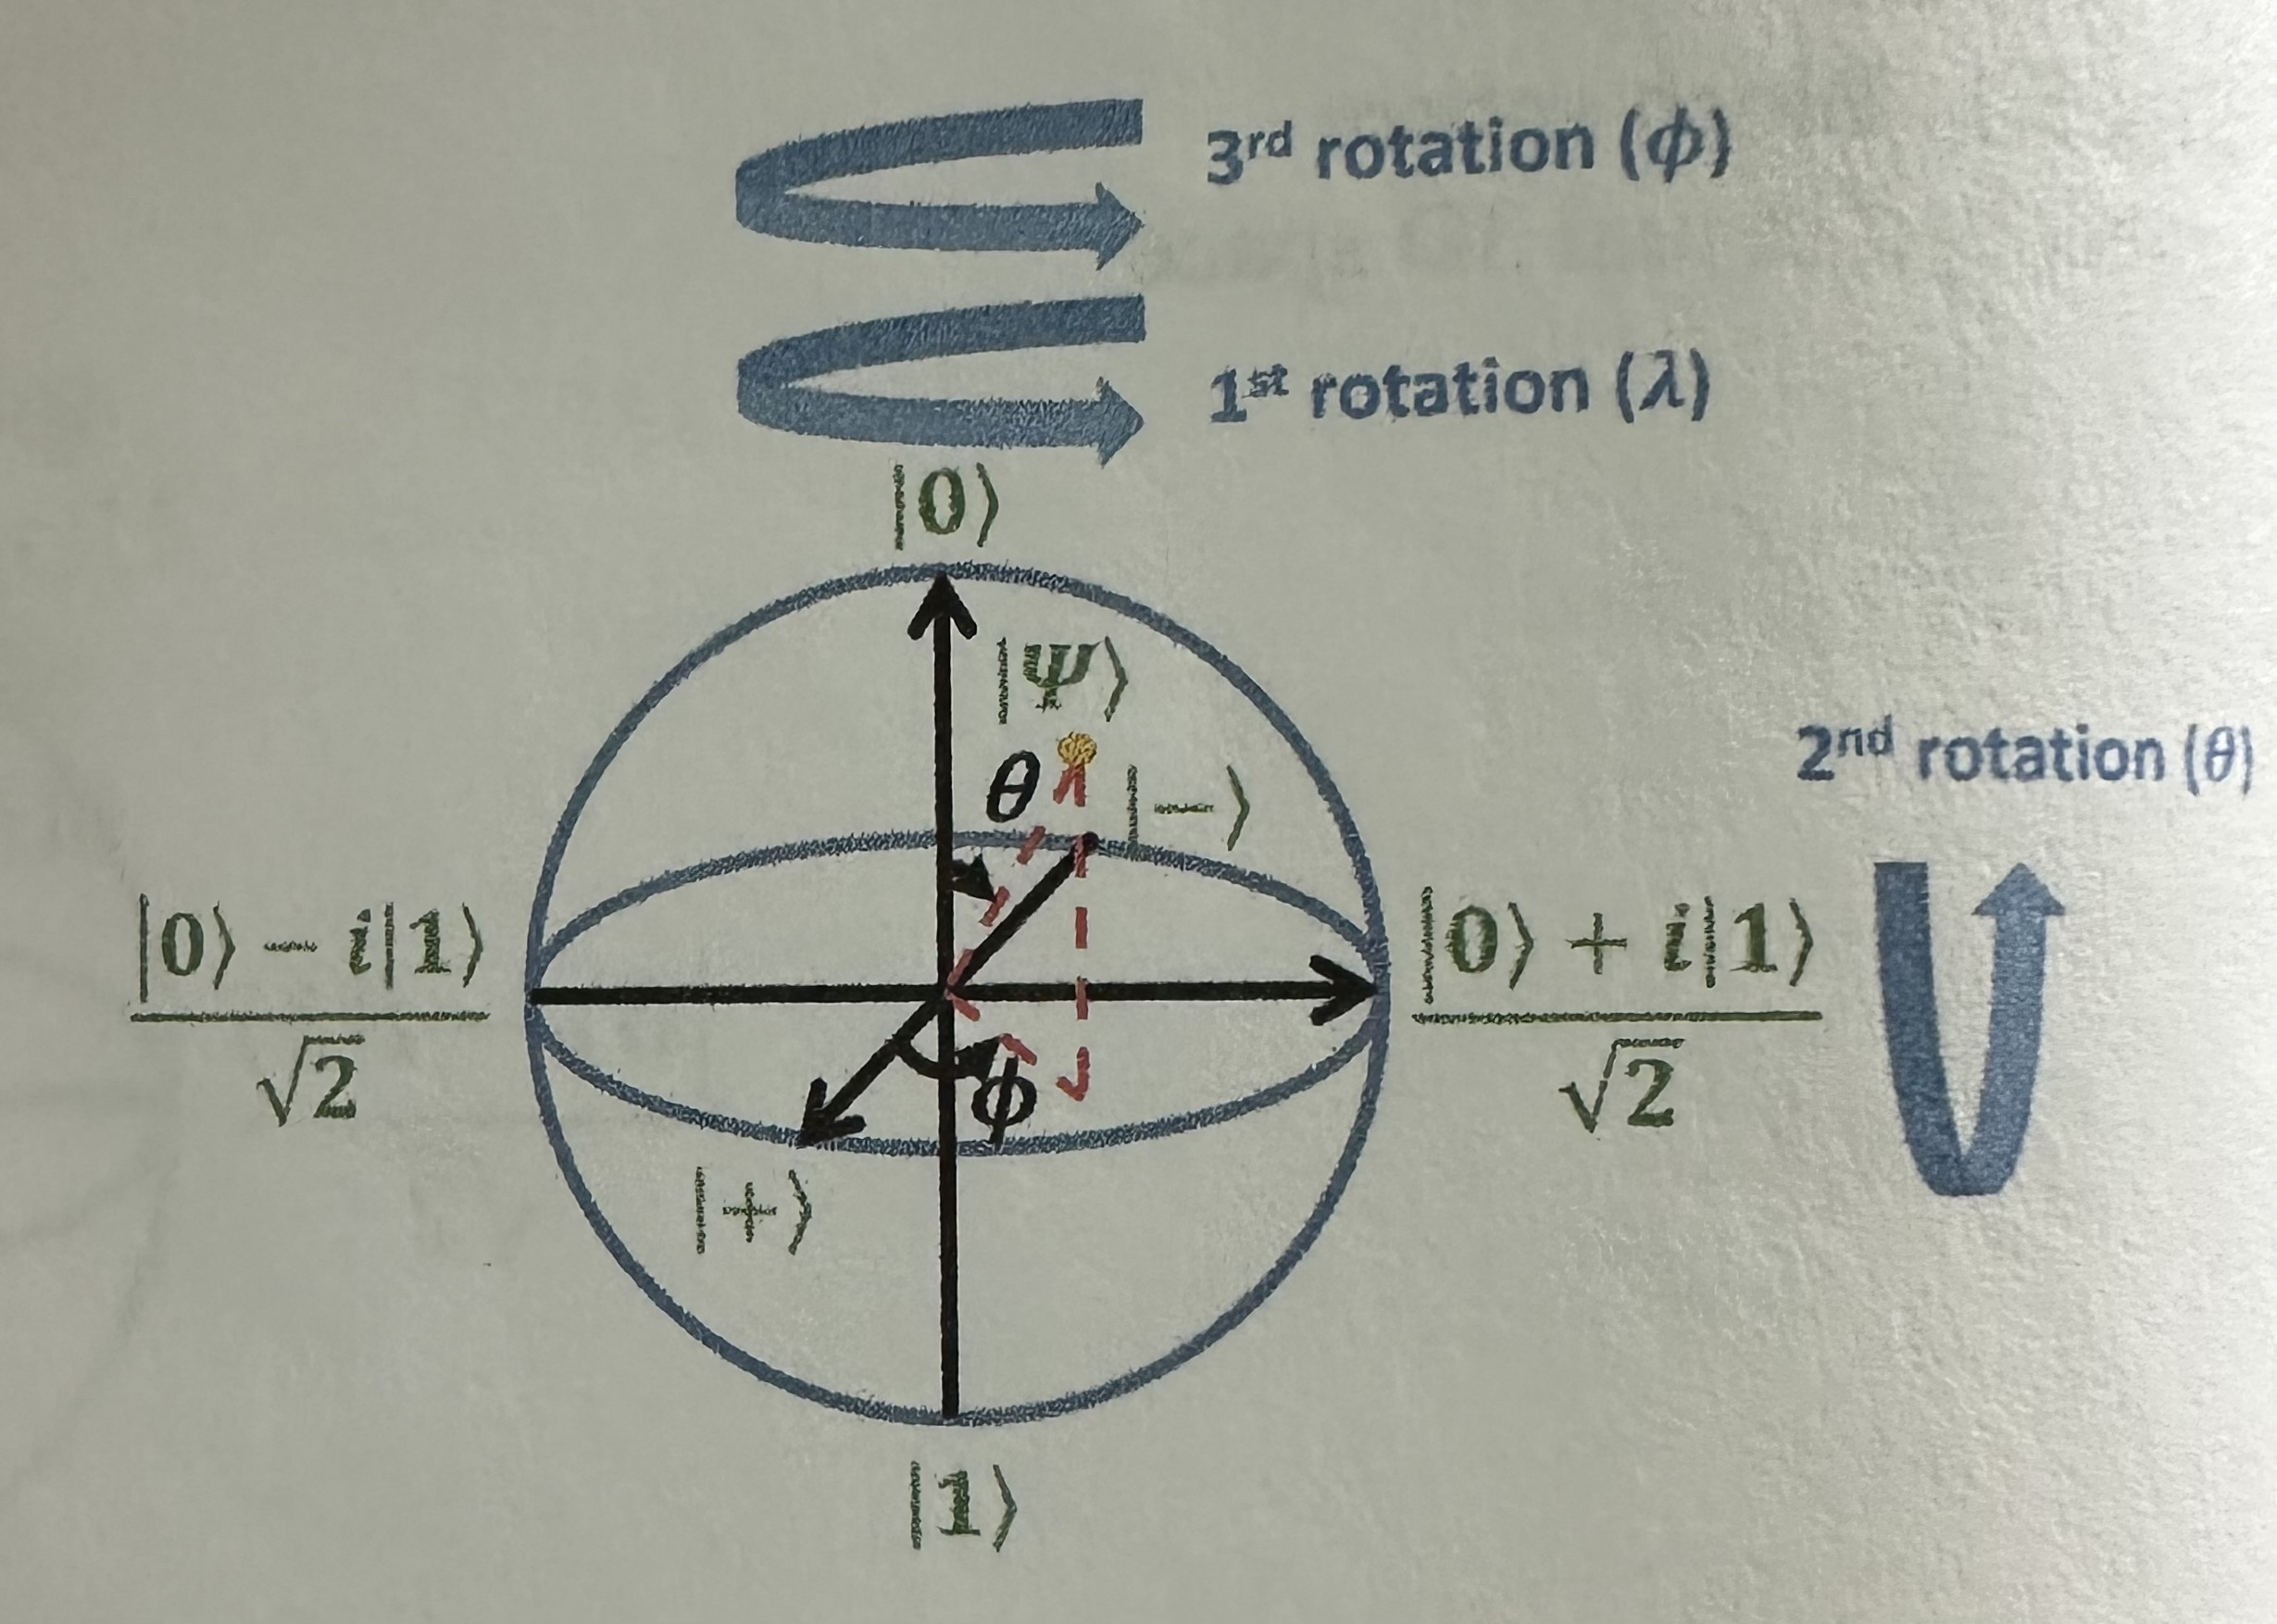
\includegraphics[scale=0.3]{Fig.5.2.jpeg}\\
\textbf{Fig. 5.1} Bloch sphere embedded in real 3D space
\end{center}
This is because complex conjugate is applied to the scalar phase associated
with the \textit{bra} (Eq.(3.5)) which cancels the extra phase from the \textit{ket}.

So, we will ignore $\gamma$, and now the qubit is described by two parameters, $\theta$, and $\phi$, with 
2 DOFs,
\begin{equation} \label{eq 5.3}
    \ket{\psi}=\cos{\frac{\theta}{2}}e^{-i\phi/2}\ket{0}+\sin{\frac{\theta}{2}}e^{i\phi/2}\ket{1}. \tag{5.3}
\end{equation}

This equation happens to map to the surface of a unit sphere, \textbf{embedded} in our
real 3D space, with $\theta$ corresponding to the \textbf{polar angle} and $\phi$
corresponding to the \textbf{azimuthal angle} on the equatorial plane. 
This allows us to visualize the hyperspace that the qubit resides in. But we need to remind
ourselves that the qubit does \textbf{not} reside in the 3D space! This unit sphere
is called the \textbf{Bloch sphere} (Fig. 5.1). Every point on the surface of the Bloch sphere corresponds to an 
infinite number of quivalent 1-qubit states which are different by only a blobal phase, $e^{i\gamma}$.
\\\\
\textbf{\large 5.3 Quantum Gate and Bloch Sphere}\\\\
Now with the introduction of the Bloch sphere, we can use it to
help us understand better how a quantum gate transforms a state. Since 
every 1-qubit state resides on the surface of the Bloch sphere,
the application of a quantum gate is just a rotation of the state
on the Bloch sphere from one point to another. An arbitary quantum gate,
\bfit{U}, corresponds to a 2 $\otimes$ 2 unitary matrix (Eq.(4.31)).
Each element in the matrix is a complex number. Therefore, there are 8 DOFs as
there are eight real parameters in the matrix (cf. Sect. 5.2). Since \bfit{U}
is unitary, its column vectors ($\ket{v_0}$ and $\ket{v_1}$) must be 
orthonormal (Eq.(3.22)) which imposes more contraints due to the three equations, namely, 
$\braket{v_0|v_0}=1, \braket{v_1|v_1} =1$, and $\braket{v_0|v_1}=0$.
The first two make sure the two column vectors are normalized.
Since they are about the norm of the vector, they only have real numbers in the
equations. So, each of them reduce the DOFs by one. For the third equation, it has
real and imaginary parts.
\begin{center}
    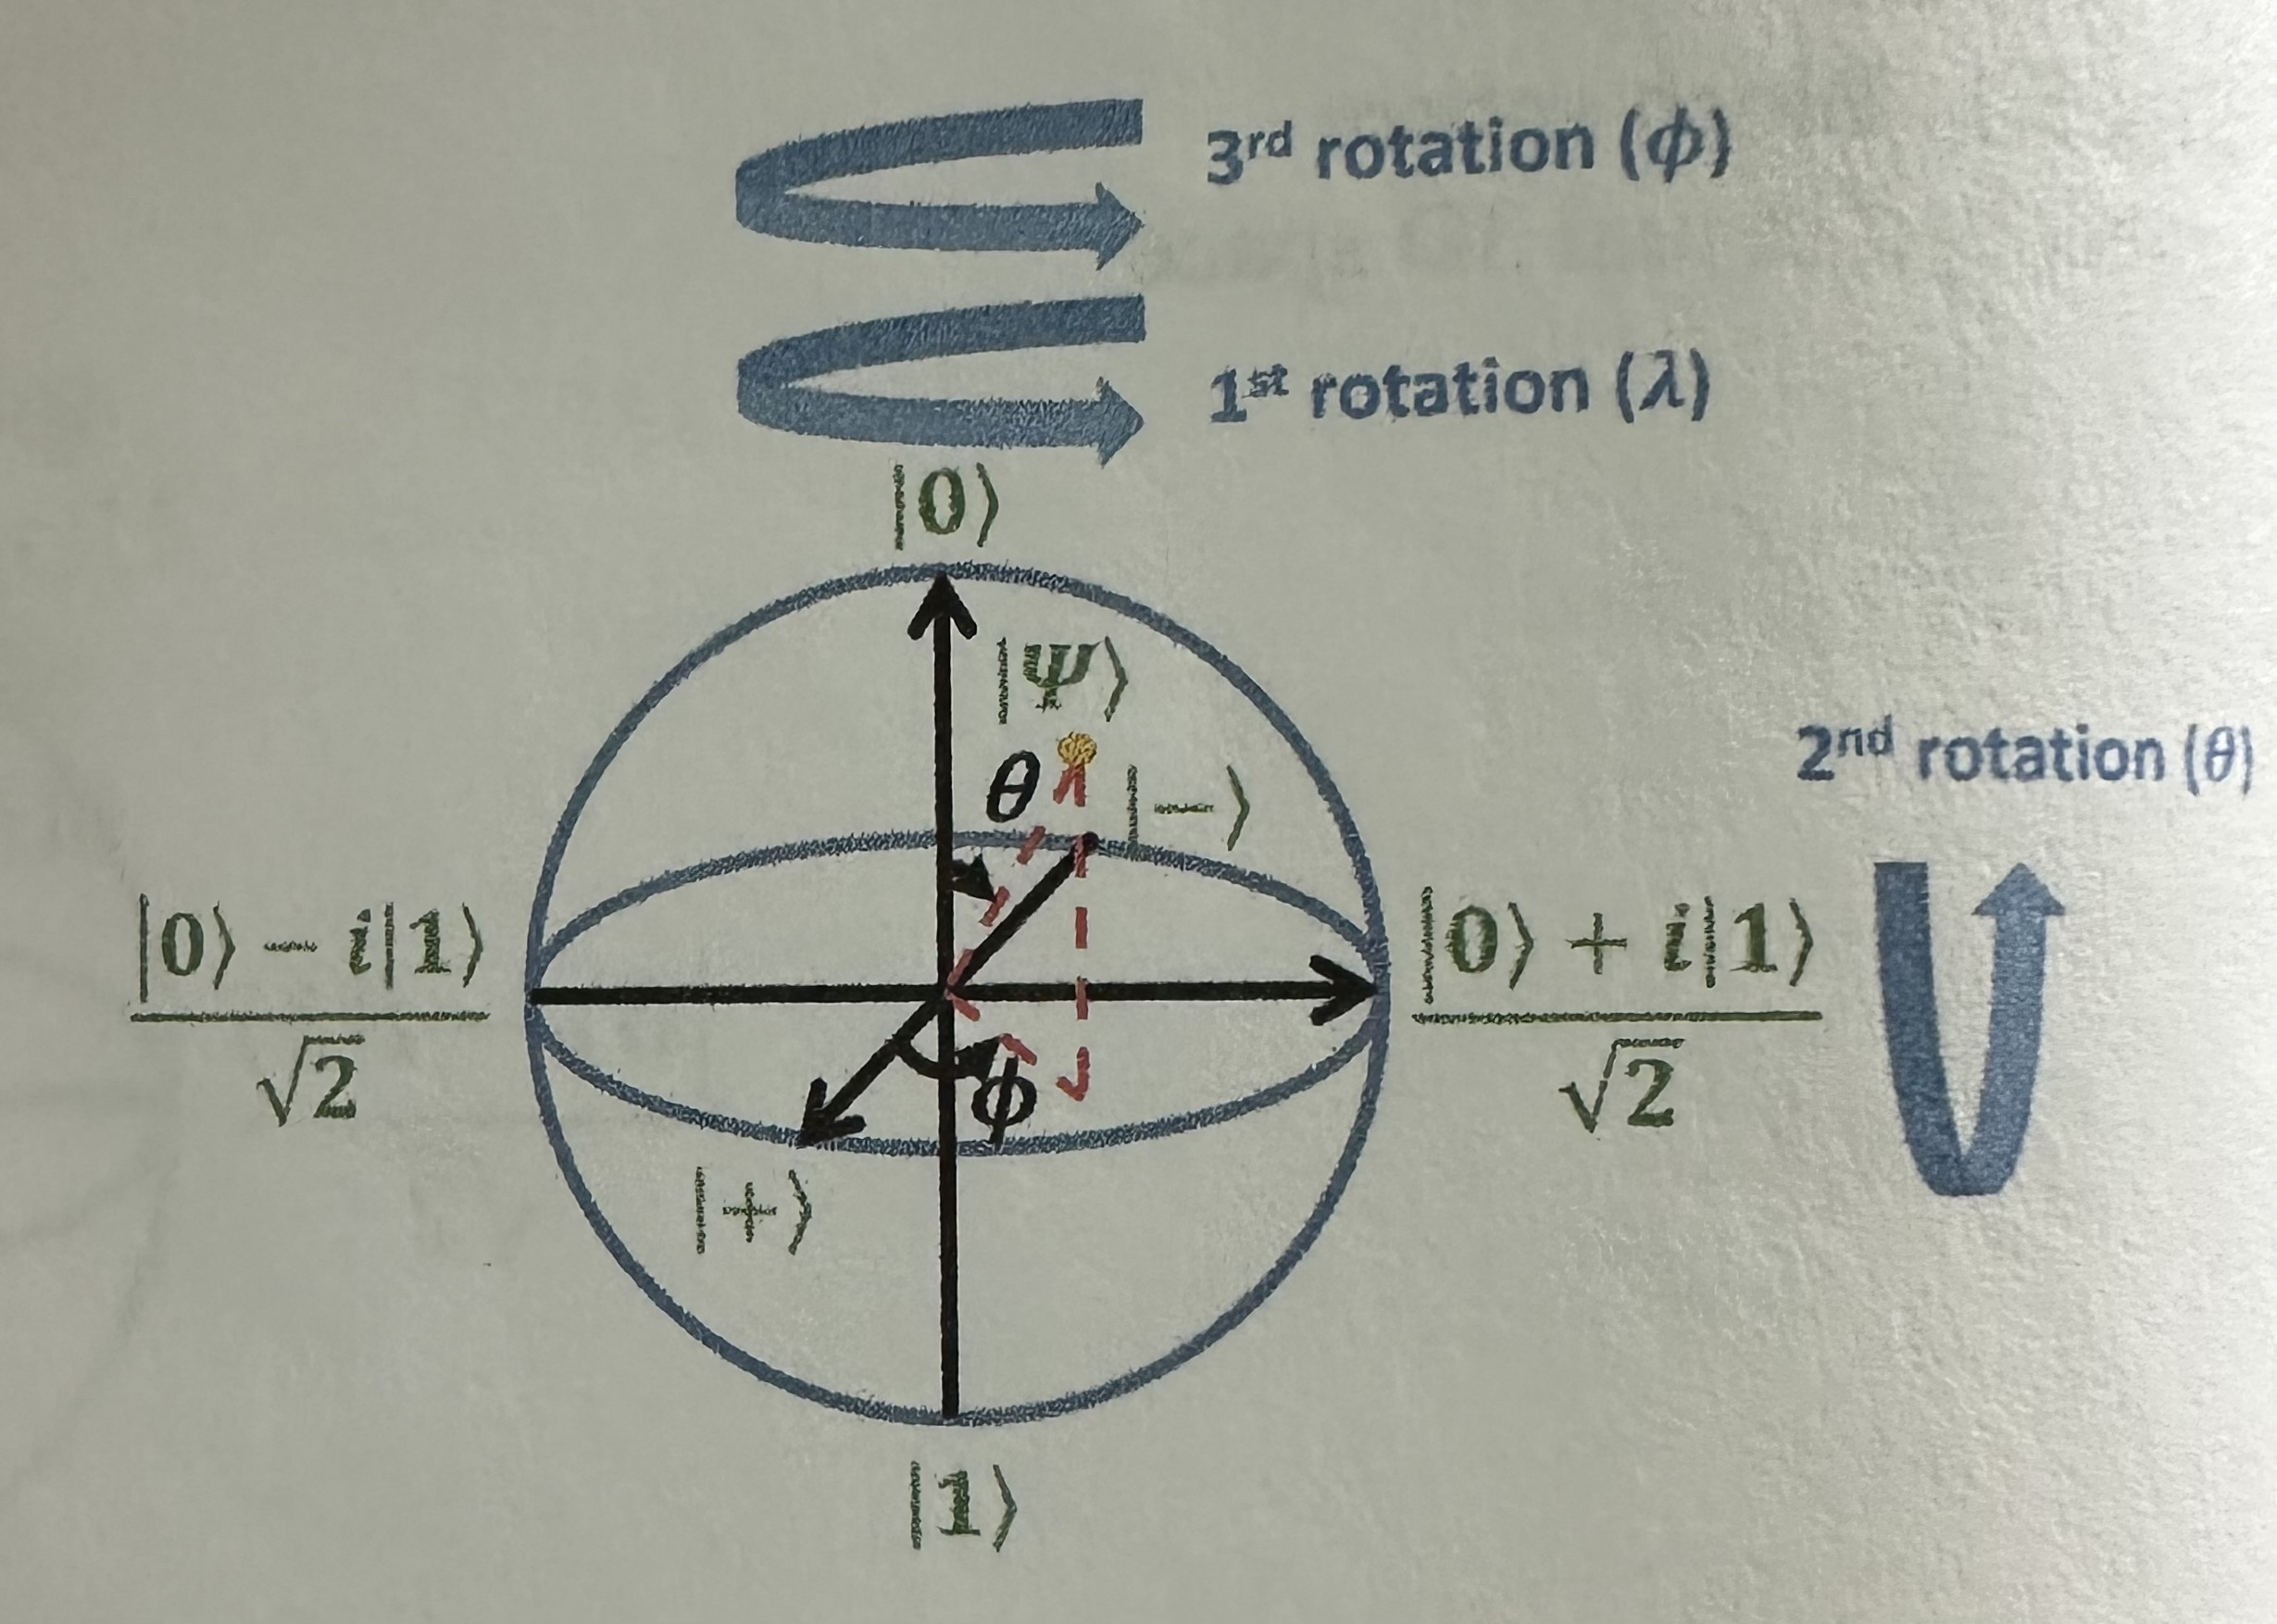
\includegraphics[scale=0.4]{Fig.5.2.jpeg}
\end{center}
\textbf{Fig. 5.2} Decomposition of any 1-qubit gate into three Euler rotations with the global phase
ignored (this is also called the "Z-Y" decomposition of a single-qubit gate)
\\
Therefore, it is equivalent to two real equations (as one needs to equate the real and imaginary
parts separately). Therefore, it reduces the DOFs by 2. As a result of being
unitary, \bfit{U} only has 4 DOFs and can be described by four parameters.
One possible representation of an arbitaray 1-qubit qunatum gate is, thus,
\begin{equation}\label{eq 5.4}
    \bfit{U}=\bfit{U}_{\boldsymbol{\theta,\phi,\lambda,\alpha}}=e^{i\alpha}\begin{pmatrix}
        \cos{\frac{\theta}{2}} & -e^{i\lambda}\sin{\frac{\theta}{2}}\\
        e^{i\phi}\sin{\frac{\theta}{2}} & e^{i(\lambda+\phi)}\cos{\frac{\theta}{2}}, \tag{5.4}
    \end{pmatrix}
\end{equation}
where it is completely described by four real parameters, $\theta, \phi, \lambda$, and $\alpha$.

This matrix corresponds to a series of three Euler rotation on the Bloch sphere and a global phase shift.
Firstly, it rotates the state about the z-axis by $\lambda$. Then it rotates
the state about the y-axis by $\theta$ followed by a rotation about the z-axis
again by $\phi$. Then it has an additional phase shift which is $e^{i\alpha}e^{i\frac{\lambda+\phi}{2}}$ (not $e^{i\alpha}$).
We will prove this in Sect. 5.5. However, since a state loses its global phase information on the
rotations corresponding to an arbitary 1-qubit gate without considering the global
phase. This is aloso called the "Z-Y" decomposition of a single-qubit gate. One may 
also perform "X-Y" decomposition (see page 176 in [1]).\\\\
\textbf{\large 5.4 Pauli Matrices}\\\\
\textbf{Pauli matrices} are very important in quantum computing. This is because Pauli
matrices are propertional to the \textbf{spin angular momentum} of a spin qubit.
Angular momentum is the \textbf{generator} of rotations (see Chapter 3 in [2]). 
The rotations turn out to be the rotatoins on the Bloch sphere embedded in the 
3D space about some given axes. We will show this later. And even if it is not a spin
qubit (such as a superconducting qubit), the problem can be transformed to use the same
framework.

There are three Pauli matrices. Since they are the operators for a 1-qubit 2D
Hilberrt space, they are 2 $\times$ 2 matrices,
\begin{equation} \label{eq 5.5}
    \sigma_x=\sigma_1=\begin{pmatrix}
        0\ 1\\ 1\ 0
    \end{pmatrix}. \tag{5.5}
\end{equation}
\begin{equation} \label{eq 5.6}
    \sigma_y=\sigma_2=\begin{pmatrix}
        0&-i\\ i & 0
    \end{pmatrix}. \tag{5.6}
\end{equation}
\begin{equation} \label{eq 5.7}
    \sigma_z=\sigma_3=\begin{pmatrix}
        1& 0\\ 0& -1
    \end{pmatrix}. \tag{5.7}
\end{equation}
We also labe $\sigma_x, \sigma_y$, and $\sigma_z$ as $\sigma_1, \sigma_2$, and $\sigma_3$
,respectively, because this is convenient for indexing.

They have the following basic properties. Firstly, they are Hermitian. This is also
expected when I tell you that Pauli matrices are propertional to the spin angular
momentum of a spin qubit, which is an obeservable (see Sect. 3.4). Therefore,
\begin{equation} \label{eq 5.8}
    \sigma_i=\sigma_i^{\dagger} \ \  (i=1,2,3).\tag{5.8}
\end{equation}
Secondly,
\begin{equation} \label{eq 5.9}
    \sigma_i^2=\sigma_i\sigma_i=\bfit{I} \ \ (i=1,2,3). \tag{5.9}
\end{equation}

\bfit{\large 5.4.1 Commutation Relation}\\\\
Paulimatrices do \textit{not} commute with each other. Together with Eq. (\ref{eq 5.9}),
it has the following \textbf{commutation} property:
\begin{equation} \label{eq 5.10}
    [\boldsymbol{\sigma_l},\boldsymbol{\sigma_m}]=\boldsymbol{\sigma_l}\boldsymbol{\sigma_m}-\boldsymbol{\sigma_m}\boldsymbol{\sigma_l}=\sum_{n}^{}2i\epsilon_{lmn}\boldsymbol{\sigma_n}. \tag{5.10}
\end{equation}
$\epsilon_{lmn}$ is the \textbf{Levi-Civita} symbol. Sometimes we can also write Eq. (5.10)
without the summation but require \textit{n} to be \textit{different from l and m}. The indices \textit{l, m,} and \textit{n}
can be any of the values of 1,2, or 3, such as $\epsilon_{223}, \epsilon_{132}, \epsilon_{123}$, etc. If
two of the indices are the same (e.g., $l=m=2$ in $\epsilon_{223}$), then it is zero (i.e., $\epsilon_{223}=0$).
Otherwise, it is $-1$ if $lmn$ can be obtained by an odd number of pair exchanges in "123".
It is 1 if $lmn$ can be obtained by an even number of pair exchnages in "123".
For example, $\epsilon_{123}$ is obtained by 1 (odd number) pair exchange in 123 by swapping
"2" and "3". Therefore, $\epsilon_{132}=-1$. But $\epsilon_{123}$ is obtained by 0 (even number) pair exchanges in 
"123". Therefore, $\epsilon_{123}=1$.\\\\
\textbf{Example 5.1} Find $\epsilon_{xyz}, \epsilon_{xzy}, \epsilon_{zxy}$, and $\epsilon_{yxz}$

Firstly, x, y, and z correspond to 1, 2, and 3, respectively (Eq.(\ref{eq 5.5})) to Eq.(\ref{eq 5.7}).
Therefore,
\begin{align} \label{eq 5.11}
    \begin{split}
        \epsilon_{xyz}&=\epsilon_{123}=1,\\
        \epsilon_{xzy}&=\epsilon_{132}=-1,\\
        \epsilon_{zxy}&=\epsilon_{312}=1,\\
        \epsilon_{yxz}&=\epsilon_{213}=-1,
    \end{split} \tag{5.11}
\end{align}
where the question is structured in a way such that each line has an extra pair of 
exchange from the previous line.
\\\\
\textbf{Example 5.2} Find $[\boldsymbol{\sigma_x},\boldsymbol{\sigma_y}]$,

Based on Eq. (5.10) and by using x, y, and z directly,
\begin{align} \label{eq 5.12}
    \begin{split}
        [\boldsymbol{\sigma_x},\boldsymbol{\sigma_y}]&=\boldsymbol{\sigma_x}\boldsymbol{\sigma_y}-\boldsymbol{\sigma_y}\boldsymbol{\sigma_x},\\
        &= 2i\epsilon_{xyz}\boldsymbol{\sigma_z},\\
        &= 2i\boldsymbol{\sigma_z}. 
    \end{split} \tag{5.12}
\end{align}

We may further slow that this is true by using matrix multiplications.
\begin{align} \label{eq 5.13}
    \begin{split}
        \boldsymbol{\sigma_x}\boldsymbol{\sigma_y}-\boldsymbol{\sigma_y}\boldsymbol{\sigma_x}&=
        \begin{pmatrix}
            0 \ 1 \\ 1\ 0
        \end{pmatrix}
        \begin{pmatrix}
            0 & -i\\ i & 0
        \end{pmatrix}-
        \begin{pmatrix}
            0 &-i\\i&0
        \end{pmatrix}
        \begin{pmatrix}
            0\ 1\\ 1\ 0
        \end{pmatrix},\\
        &=\begin{pmatrix}
            i &0\\0& -i
        \end{pmatrix}-
        \begin{pmatrix}
            -i& 0\\0&i
        \end{pmatrix}.\\
        &=\begin{pmatrix}
            2i&0\\0&-2i
        \end{pmatrix},\\
        &=2i\boldsymbol{\sigma_z}.
    \end{split} \tag{5.13}
\end{align}

When $l=m$, then $\epsilon_{lmn}=0$ and [$\boldsymbol{\sigma_l},\boldsymbol{\sigma_m}]=0$. That means it commutes with itself as 
$\boldsymbol{\sigma_l}\boldsymbol{\sigma_m}=\boldsymbol{\sigma_l}\boldsymbol{\sigma_l}=\boldsymbol{\sigma_m}\boldsymbol{\sigma_l}$.
\\\\
\bfit{\large 5.4.2 Anti-commutation Relation}\\\\
Pauli matrices anti-commute with the other. That means $\boldsymbol{\sigma_l}\boldsymbol{\sigma_m}+\boldsymbol{\sigma_m}\boldsymbol{\sigma_l}=0$ if
$l\neq m$. If $l=m$, then it is just two times of \bfit{I} due to Eq.(\ref{eq 5.9}). Their
anti-commutation relation can be summarized as,
\begin{equation} \label{eq 5.14}
    [\boldsymbol{\sigma_l},\boldsymbol{\sigma_m}]=\boldsymbol{\sigma_l\sigma_m}+\boldsymbol{\sigma_m\sigma_l}=2\delta_{lm}\bfit{I},\tag{5.14}
\end{equation}
where we have used the \textbf{Kronechker delta} symbol (Eq.(2.23)).
\\
\textbf{Example 5.3} Find [\textbf{$\sigma_x$},\textbf{$\sigma_y$}] using matrix multipication.
\begin{align} \label{eq 5.15}
    \begin{split}
        [\boldsymbol{\sigma_x}, \boldsymbol{\sigma_y}]&=\boldsymbol{\sigma_x\sigma_y}+\boldsymbol{\sigma_y\sigma_x},\\
        &=\begin{pmatrix}
            0\ 1\\1\ 0
        \end{pmatrix}
        \begin{pmatrix}
            0 &-i\\ i& 0
        \end{pmatrix}+
        \begin{pmatrix}
            0& -i\\ i& 0
        \end{pmatrix}
        \begin{pmatrix}
            0\ 1 \\ 1\ 0
        \end{pmatrix},\\
        &=\begin{pmatrix}
            i & 0\\ 0& -i
        \end{pmatrix}+
        \begin{pmatrix}
            -i & 0\\ 0& i
        \end{pmatrix},\\
        &=\begin{pmatrix}
            0\ 0\\ 0\ 0
        \end{pmatrix}\\
        &= \textbf{0}.
    \end{split} \tag{5.15}
\end{align}
\hfill $\blacksquare$
\\\\
\bfit{\large 5.4.3 Trace Properties}\\\\
Pauli matrices are traceless. The trace of a matrix is the sum of the diagonal
elements. A traceless matrix is a matrix with zero trace,
\begin{equation}\label{eq 5.16}
    tr(\boldsymbol{\sigma_i})=0 \ \ (i=1,2,3).\tag{5.16}
\end{equation}
\\\\
\textbf{Example 5.4} Show that $\boldsymbol{\sigma_z}$ is traceless.
\begin{equation}\label{eq 5.17}
    tr(\boldsymbol{\sigma_z})=tr\begin{pmatrix}
        1& 0\\ 0& -1
    \end{pmatrix}= 1 + (-1)=0.\tag{5.17}
\end{equation}
Therefore, $\boldsymbol{\sigma_z}$ is traceless.

How about the trace of the product of Pauli matrices, tr($\boldsymbol{\sigma_l\sigma_m})$?
Again, $l$ and $m$ can be any of  x, y, and z (or 1, 2, and 3). It is given by the following equation:
\begin{equation}\label{eq 5.18}
    tr(\boldsymbol{\sigma_l\sigma_m})=2\delta_{lm}. \tag{5.18}
\end{equation}
This means that any product of two different Pauli matrices is \textit{traceless}. \
Let us prove Eq. (\ref{eq 5.18}).
\\
\textbf{Example 5.5} Prove Eq. (\ref{eq 5.18}).

To be more instructive, we will prove by considering $l=m$ and $l\neq m$ seperately.
Firstly, we express it in terms of the commutator and anti-commutator,
\begin{equation} \label{eq 5.19}
    \boldsymbol{\sigma_l\sigma_m}=\frac{[\boldsymbol{\sigma_l},\boldsymbol{\sigma_m}]+[\boldsymbol{\sigma_l},\boldsymbol{\sigma_m}]}{2}.\tag{5.19}
\end{equation}

When $l=m, \delta_{lm}=1$ and $\epsilon_{lmn}=0$. Based on Eqs. (\ref{eq 5.10}) and (\ref{eq 5.14}),
\begin{equation}\label{eq 5.20}
    \boldsymbol{\sigma_l\sigma_m}=\frac{\textbf{0}_2\bfit{I}}{2}=\bfit{I}=\begin{pmatrix}
        1\ 0\\ 0\ 1
    \end{pmatrix}. \tag{5.20}
\end{equation}
Therefore, tr($\boldsymbol{\sigma_l\sigma_m})=$ tr(\bfit{I})$=1+1=2$ and
Eq. (\ref{eq 5.18}) is correct.

Now consider when $l\neq m$. Then $\delta_{lm}=0$.
\begin{equation}\label{eq 5.21}
    \boldsymbol{\sigma_l\sigma_m}=\frac{2i\epsilon_{lmn}\boldsymbol{\sigma_n}+\boldsymbol{0}}{2}=\frac{2i\epsilon_{lmn}\boldsymbol{\sigma_n}}{2}.\tag{5.21}
\end{equation}
This does not give us the answer but we only care about the trace. Therefore,
\begin{align}\label{eq 5.22}
    \begin{split}
        tr(\boldsymbol{\sigma_l\sigma_m})&=tr(\frac{2i\epsilon_{lmn}\boldsymbol{\sigma_n}}{2}),\\
        &=\frac{2i\epsilon_{lmn}}{2}tr(\boldsymbol{\sigma_n}),\\
        &=0.
    \end{split} \tag{5.22}
\end{align}
where in line 3, we have used the fact that Pauli matrices are traceless (Eq. (\ref{eq 5.16})). 
And again, Eq. (\ref{eq 5.18}) is correct. \hfill $\blacksquare$
\\\\
\textbf{\large 5.5 Universal Sets of Gates}\\\\
Now we will discuss the idea of universal stes of quantum gates based on [1] with
variations. This is similar to classical logic. In classical logic, any logical operation can be 
broken dwon into some eniversal sets of gates. For example, the set of NOT gate and AND gate
(so only 2) can contruct any logic. Constructing the circuit using a set of universal gates makes logic synthesis
easier and also allow optimization on a limited set of gates. This is the same for quantum computing.
If we can decompose all gates into a finite number of gates, efforts can be spent on optimizing those gates 
(e.g., to achieve the bes microwave pulse shapes corresponding to the gates
in the set). Moreover, we also wanat to use the gates that work with error correction.

We already kwno that every 1-qubit gate may be described by four parameters through
Eq. (\ref{eq 5.4}). We claim that it can be decomposed into three rotations in Fig. 5.2 followed by a global
phase shift. It turns out that spin angular momentum is the generator of rotation
on the Bloch sphere. We will not discuss the meaning of "generator". Readers can refer to 
Chapter 3 in [2]. We will take it for granted. Since the Pauli matrices are propertional to spin
angular momenta about the $\hat{x}, \hat{y},$ and $\hat{z}$ axes, respectively, they can be used to create
(generate) the corresponding rotation matrices. The rotation matrices about $\hat{l}, \bfit{R}_l(\boldsymbol{\theta})$, for $l=x, y, z,$ are
\begin{align}
    \label{eq 5.23}&\bfit{R}_{\boldsymbol{x}}(\theta)= e^{-i\theta\boldsymbol{\sigma_x}/2}=\cos{\frac{\theta}{2}}\bfit{I}-i\sin{\frac{\theta}{2}\boldsymbol{\sigma_x}}=\begin{pmatrix}
        \cos{\frac{\theta}{2}}&-i\sin{\frac{\theta}{2}}\\
        -i\sin{\frac{\theta}{2}}&\cos{\frac{\theta}{2}}
    \end{pmatrix},\tag{5.23}\\
   \label{eq 5.24} &\bfit{R}_{\boldsymbol{y}}(\theta)= e^{-i\theta\boldsymbol{\sigma_y}/2}=\cos{\frac{\theta}{2}}\bfit{I}-i\sin{\frac{\theta}{2}\boldsymbol{\sigma_y}}=\begin{pmatrix}
        \cos{\frac{\theta}{2}}&\sin{\frac{\theta}{2}}\\
        \sin{\frac{\theta}{2}}&\cos{\frac{\theta}{2}}
    \end{pmatrix},\tag{5.24}\\ 
    \label{eq 5.25}&\bfit{R}_{\boldsymbol{z}}(\theta)= e^{-i\theta\boldsymbol{\sigma_z}/2}=\cos{\frac{\theta}{2}}\bfit{I}-i\sin{\frac{\theta}{2}\boldsymbol{\sigma_z}}=\begin{pmatrix}
        e^{-i\frac{\theta}{2}}&0\\
       0&e^{i\frac{\theta}{2}}
    \end{pmatrix},\tag{5.23}
\end{align}

The exponential terms, $e^{-i\theta\boldsymbol{\sigma_l}/2}$, in Eq. (\ref{eq 5.23}) and Eq. (5.25) have
the form of $e^{-i\frac{H}{\hbar}t}$ as in Eq. (4.31). Therefore, we need to find a Hamiltonian that is propertional to
the Pauli matrices to perform rotations and this will be discussed when we study the actual implementation.

It can be shown that the matrix in Eq. (\ref{eq 5.4}) can be decomposed into
\begin{align*} \label{eq 5.26}
    \bfit{U}_{\boldsymbol{\theta},\boldsymbol{\phi},\boldsymbol{\lambda},\boldsymbol{\alpha}}&=e^{i\alpha}\begin{pmatrix}
        \cos{\frac{\theta}{2}}&-e^{i\lambda}\sin{\frac{\theta}{2}}\\
        e_{i\phi}\sin{\frac{\theta}{2}}& e^{i(\lambda+\phi)}\cos{\frac{\theta}{2}}
    \end{pmatrix},\\
    &=e^{i\alpha}e^{i\frac{\lambda+\phi}{2}}\bfit{R}_{\bfit{z}}(\phi)\bfit{R}_{\bfit{y}}(\theta)\bfit{R}_{\bfit{z}}(\lambda),\\
    &=e^{i\alpha^\prime}\bfit{R}_{\bfit{z}}(\phi)\bfit{R}_{\bfit{y}}(\theta)\bfit{R}_{\bfit{z}}(\lambda). \tag{5.26}
\end{align*}

Therefore, to implement any 1-qubit gate, we only need to be able to
perform a rotation about the $\hat{z}$ and$\hat{y}$ for an arbitary angle
and implement a global phase shifter. THe global phase shifter can be denoted as an operator
as $e^{i\alpha^\prime} \boldsymbol{I}$, where $\alpha_\prime$ is the total global phase in Eq. (\ref{eq 5.26}).

However, we also need to perform entnaglement operations for 2 or more qubits.
We need a 2-qubit CNOT gate, \bfit{U}$_{\boldsymbol{X O R}}$ (Eq. (4.49)). Moreover,
in order to implement controlled operations, \bfit{R}$_{\boldsymbol{x}}$ is also required (see CHapter 4 in [1]).
Therefore, one of the \textbf{universal sets of quantum gate} is $\{ e^{i\alpha^\prime}\boldsymbol{I}, \boldsymbol{R_x}(\theta_x),
\boldsymbol{R_z}(\theta_y),$ $\boldsymbol{R_z}(\theta_z),\boldsymbol{U}_{\boldsymbol{X O R}} \}$.

Although there are only five types of gates in this set of quantum gates, four of them are \textit{continuous}
due to the continuous parameters, $\alpha^\prime, \theta_x, \theta_y,$ and $\theta_z$.
So, strictly speaking, we still need to be able to implement infinite numbers of gates, although
the number of types is limited to 5.

It is also possible to derive a universal set of quantum gates without continuous
parameters. This set contains $\{ \boldsymbol{H, S, T, U}_{\boldsymbol{X O R}} \}$ (see 
also Eq. (4.43) and (4.44)). However, they are \textit{not} exact. But they can infinitely
approximate any quantum gates.
\\\\
\bfit{\large 5.5.1 Some Useful Mathematics}\\\\
It will be instructive to show Eqs. (\ref{eq 5.26}) and (5.23) to (5.25) are correct,
through which we will practice some important skills.\\\\
\textbf{Example 5.6} Prove Eq. (\ref{eq 5.26}).

This is just a simple matrix multiplication and we will work backward.
\begin{align*}\label{eq 5.27}
    &e^{i\alpha}e^{i\frac{\lambda+\phi}{2}}\boldsymbol{R_z}(\phi)\boldsymbol{R_y}(\theta)\boldsymbol{R_z}(\lambda),\\
    =&e^{i\alpha}e^{i\frac{\lambda+\phi}{2}}
    \begin{pmatrix}
        e^{-i\frac{\phi}{2}}&0\\0&e^{i\frac{\phi}{2}}
    \end{pmatrix}
    \begin{pmatrix}
        \cos{\frac{\theta}{2}}& -\sin{\frac{\theta}{2}}\\
        \sin{\frac{\theta}{2}}&\cos{\frac{\theta}{2}}
    \end{pmatrix}
    \begin{pmatrix}
        e^{-i\frac{\lambda}{2}}&0\\0&e^{i\frac{\lambda}{2}}
    \end{pmatrix},\\
    =&e^{i\alpha}e^{i\frac{\lambda+\phi}{2}}
    \begin{pmatrix}
        e^{-i\frac{\phi}{2}}&0\\0&e^{i\frac{\phi}{2}}
    \end{pmatrix}
    \begin{pmatrix}
        e^{-i\frac{\lambda}{2}}\cos{\frac{\theta}{2}}&-e^{i\frac{\lambda}{2}}\sin{\frac{\theta}{2}}\\
        e^{-i\frac{\lambda}{2}}\sin{\frac{\theta}{2}}&e^{i\frac{\lambda}{2}}\cos{\frac{\theta}{2}}
    \end{pmatrix},\\
    =&e^{i\alpha}e^{i\frac{\lambda+\phi}{2}}\begin{pmatrix}
        e^{-i\frac{\lambda+\phi}{2}}\cos{\frac{\theta}{2}}&-e^{i\frac{\lambda-\phi}{2}}\sin{\frac{\theta}{2}}\\
        e^{-i\frac{\lambda-\phi}{2}}\sin{\frac{\theta}{2}}&e^{i\frac{\lambda+\phi}{2}}\cos{\frac{\theta}{2}}
    \end{pmatrix},\\
    =&e^{i\alpha}\begin{pmatrix}
        \cos{\frac{\theta}{2}}&-e^{i\lambda}\sin{\frac{\theta}{2}}\\
        e^{i\phi}\sin{\frac{\theta}{2}}&e^{i(\lambda+\phi)}\cos{\frac{\theta}{2}}
    \end{pmatrix}. \tag{5.27}
\end{align*}
\hfill $\blacksquare$\\\\
\textbf{Example 5.7} Prove Eq. (5.24).\\\\
We will first show $e^{i\theta\boldsymbol{\sigma_y}/2}=\cos{\frac{\theta}{2}}\boldsymbol{I}-i\sin{\frac{\theta}{2}}\boldsymbol{\sigma_y}$.
We first express the matrix exponential in the form similar to the sin and cos functions ($\sin{x}=\frac{e^{ix}-e^{-ix}}{2o}$ and
$\cos{x}=\frac{e^{ix}+e^{-ix}}{2}$),
\begin{equation}\label{eq 5.28}
    e^{-i\theta\boldsymbol{\sigma_y}/2}=\frac{e^{-i\theta\boldsymbol{\sigma_y}/2}+e^{i\theta\boldsymbol{\sigma_y}/2}}{2}+
    \frac{e^{-i\theta\boldsymbol{\sigma_y}/2}-e^{i\theta\boldsymbol{\sigma_y}/2}}{2}, \tag{5.28}
\end{equation}
which is composed of a sum term and a difference term. Now, we will use the Taylor
expansion of matrix exponential as in Eq. (4.18),
\begin{equation}\label{eq 5.29}
    e^{-i\theta\boldsymbol{\sigma_y}/2}=\sum_{k=0}^{\infty}\frac{(-i\theta\boldsymbol{\sigma_y}/2)^k}{k!},\tag{5.29}
\end{equation}
\begin{equation}\label{eq 5.30}
     e^{i\theta\boldsymbol{\sigma_y}/2}=\sum_{k=0}^{\infty}\frac{(i\theta\boldsymbol{\sigma_y}/2)^k}{k!}.\tag{5.30}
\end{equation}
These two equations are the same except that the terms with odd $k$ have different
sign in Eqs. (\ref{eq 5.29}) and (\ref{eq 5.30}). Therefore, for the sum term in Eq. (\ref{eq 5.28}),
only even $k$ terms are left. So,
\begin{align*}\label{eq 5.31}
    &\frac{e^{-i\theta\boldsymbol{\sigma_y}/2}+e^{i\theta\boldsymbol{\sigma_y}/2}}{2}\\
    =&\frac{1}{2}\left[ \frac{2(-i\theta\boldsymbol{\sigma_y}/2)^0}{0!}+\frac{2(-i\theta\boldsymbol{\sigma_y}/2)^2}{2!}+\frac{2(-i\theta\boldsymbol{\sigma_y})^4}{4!}+\cdots \right], \\
    =&\left[\frac{(-i\theta/2)^0}{0!}+\frac{(-i\theta/2)^2}{2!}+\frac{(-i\theta/2)^4}{4!}+\cdots\right]\bfit{I},\\
    =&\left[\frac{(\theta/2)^0}{0!}-\frac{(\theta/2)^2}{2!}+\frac{(\theta/2)^4}{4!}+\cdots\right]\bfit{I},\\
    =&\cos{\frac{\theta}{2}}\bfit{I},\tag{5.31}
\end{align*}
where we have used the fact that $\boldsymbol{\sigma_y\sigma_y}=\boldsymbol{I}$ from the line 2 to line 3 (Eq. (\ref{eq 5.9})).
As a result, any even power of $\boldsymbol{\sigma_y}$ is \bfit{I}.

And for the difference term in Eq. (\ref{eq 5.28}), only odd $k$ terms are left. So,
\begin{align*}\label{eq 5.32}
    &\frac{e^{-i\theta\boldsymbol{\sigma_y}/2}-e^{i\theta\boldsymbol{\sigma_y}/2}}{2}\\
    =&\frac{1}{2}\left[ \frac{2(-i\theta\boldsymbol{\sigma_y}/2)^1}{1!}+\frac{2(-i\theta\boldsymbol{\sigma_y}/2)^3}{3!}+\frac{2(-i\theta\boldsymbol{\sigma_y})^5}{5!}+\cdots \right], \\
    =&\left[\frac{(-i\theta/2)^1}{1!}+\frac{(-i\theta/2)^3}{3!}+\frac{(-i\theta/2)^5}{5!}+\cdots\right]\boldsymbol{\sigma_y},\\
    =&-i\left[\frac{(\theta/2)^1}{1!}-\frac{(\theta/2)^3}{3!}+\frac{(\theta/2)^5}{5!}+\cdots\right]boldsymbol{\sigma_y},\\
    =&i\sin{\frac{\theta}{2}}\boldsymbol{\sigma_y},\tag{5.32}
\end{align*}
where we used $\boldsymbol{\sigma_y\sigma_y}=\boldsymbol{I}$ again. But since each term has an old
power of $\boldsymbol{\sigma_y}$, they are all evaluated to be $\boldsymbol{\sigma_y}$, instead of \bfit{I}.
Therefore, we have proved $e^{i\theta\boldsymbol{\sigma_y}/2}=\cos{\frac{\theta}{2}\boldsymbol{I}}-i\sin{\frac{\theta}{2}}\boldsymbol{\sigma_y}$.

Now, we will prove $\cos{\frac{\theta}{2}}\boldsymbol{I}-i\sin{\frac{\theta}{2}}\boldsymbol{\sigma_y}=\begin{pmatrix}
    \cos{\frac{\theta}{2}}& -\sin{\frac{\theta}{2}}\\
    \sin{\frac{\theta}{2}}& \cos{\frac{\theta}{2}}
\end{pmatrix}$. This is straighforward by just performing matrix addition,
\begin{align*}\label{eq 5.33}
    &\cos{\frac{\theta}{2}}\boldsymbol{I}-i\sin{\frac{\theta}{2}}\boldsymbol{\sigma_y},\\
    =&\cos{\frac{\theta}{2}}\begin{pmatrix}
        1\ 0\\ 0\ 1
    \end{pmatrix}-
    i\sin{\frac{\theta}{2}}\begin{pmatrix}
        0& -i\\ i& 0
    \end{pmatrix},\\
    =&\begin{pmatrix}
        \cos{\frac{\theta}{2}}&0\\0&\cos{\frac{\theta}{2}}
    \end{pmatrix}+
    \begin{pmatrix}
        0& -\sin{\frac{\theta}{2}}\\ \sin{\frac{\theta}{2}}&0
    \end{pmatrix},\\
    =&\begin{pmatrix}
        \cos{\frac{\theta}{2}} & -\sin{\frac{\theta}{2}}\\
        \sin{\frac{\theta}{2}} & \cos{\frac{\theta}{2}}
    \end{pmatrix}. \tag{5.33}
\end{align*}
\hfill $\blacksquare$\\\\
\textbf{\large 5.6 Summary}\\\\
If we ignore the global phase, due to the normalization requirement,
a 1-qubit state can be described by two real parameters. As a result, we can
map the 2D complex space to the Bloch sphere surface which can be embedded in the real 
3D space. The Bloch sphere provides a lot of convenience for our understanding of qubit manipulation.
For example, any 1-qubit gate can be described by four real parameters. If the global
phase is ignored again, an arbitrary 1-qubit quantum gate can be decomposed
into a rotation about the $\hat{z}$ followed by a rotation about $\hat{y}$ and 
then followed by a third rotation about $\hat{z}$. These rotations can be 
generated using Pauli matrices. We have learned some importatn properties of the 
Pauli matrices. We have also discussed that we may use $\left\{e^{i\alpha^\prime}\boldsymbol{I}, \boldsymbol{R_x}(\theta_x), \boldsymbol{R_y}(\theta_y), \boldsymbol{R_z}(\theta_y), \boldsymbol{U}_{\boldsymbol{X O R}}\right\}$
as a universal set of quantum gates. However, some of the gates have continuous parameters. If we allow approximations, 
$\left[\boldsymbol{H, S, T}, \boldsymbol{U}_{\boldsymbol{X O R}}\right]$ can be used as a
universal set of quantum gates instead.\\\\\\
\textbf{\large Problems}\\\\
\textbf{ 5.1 Qubit Gate Matrix}

Prove \bfit{U} in Eq. (\ref{eq 5.4}) is unitary.\\\\
\textbf{ 5.2 Pauli Matrices}

Prove Eqs. (\ref{eq 5.8}) and (\ref{eq 5.9}).\\\\
\textbf{5.3 Rotatio Matrices}

Prove Eqs. (\ref{eq 5.23}) and (5.25). See Sect. 5.5.1.\\\\
\textbf{5.4 Single Qubit State Representation}

Compare Eq. (\ref{eq 5.3}) to Eq. (1.4) in [1] and argue that they are equivalent.\\\\
\textbf{5.5 Rotation Matrix Representation}

Compare Eq. (\ref{eq 5.4}) to Eqs. (1.17) and (4.12) in [1] and argue that they are equivalent.\\\\
\textbf{\large References}\\\\
1. M.A. Nielsen and I. L. Chuang. \textit{Quantum Computation and Quantum Information: 10th Anniversary Edition.} Cambridge University Press, 2011.\\
2. J. J. Sakurai. \textit{Modern Quantum Mechanics.} Addison-Wesley, 1993.

\end{document}
